\documentclass{book}

\usepackage{titling}
\title{Literatuurstudie}
\author{Debaere Jens \and Simon Vanpaemel}
\usepackage[pdftitle={\thetitle},pdfauthor={\theauthor}]{hyperref}
\usepackage[dutch]{babel}
\usepackage[utf8]{inputenc}
\usepackage{amsmath, amssymb, amsthm, siunitx , graphicx, epstopdf}
\usepackage{tabularx}
%\usepackage{subfigure}
\usepackage{epstopdf}
\usepackage[export]{adjustbox}
\usepackage{colortbl}
\usepackage{tabularx}
\usepackage[table]{xcolor}
\usepackage{booktabs}
\usepackage{float}
\usepackage{xfrac}
\usepackage{fancyhdr}
\usepackage{mathabx}
\usepackage{caption}
\usepackage{subcaption}
\captionsetup{compatibility=false}
%\usepackage{gensymb}
\usepackage{lscape}
\usepackage{multicol}
\begin{document}
\chapter{Literatuurstudie}
\label{hoofdstuk:1}
\section{Inleiding}
\subsection{Wat is SLAM?}
Wanneer een robot in een ruimte losgelaten wordt is het wenselijk dat deze daar zonder begeleiding door kan navigeren. Dit kan bijvoorbeeld door de robot een voorgeprogrammeerde map mee te geven. Deze kan de robot dan vergelijken met zijn observaties om een schatting te maken van de locatie waarop hij zich bevindt. Op die manier is het mogelijk een traject te bepalen om naar een gewenste positie te navigeren.  Dit probleem staat bekend onder het "localization-problem". \\
Daarnaast kan het ook wenselijk zijn een map op te bouwen van de omgeving terwijl de robot zich door deze omgeving beweegt. Dit kan door de metingen te verwerken terwijl de robot zijn positie op elk moment kent. \\
SLAM ofwel "Simultaneous localization and Mapping" combineert deze twee problemen en probeert deze tegelijk op te lossen. Hierbij zijn dus zowel de positie als de map volledig onbekend. Een oplossing van dit probleem opent dan ook de deuren naar een volledig autonome navigatie. \\
Toepassingen hiervan kunnen teruggevonden worden in bijvoorbeeld autonome stofzuiger of grasmachines. Maar ook op industriële schaal waarin autonome heftrucks zich in een omgeving voortbewegen waarin tegelijk personen kunnen rondlopen zonder verstoring van het systeem.\cite{Course}\\

\subsection{Definitie van het probleem}
Om tot een oplossing, of tenminste een goeie benadering ervan, te komen moeten dus twee belangrijke onbekenden bepaalt worden.
\begin{enumerate}
	\item \textbf{De kaart van de omgeving: }$m$
	\item \textbf{Het pad van de robot: }Vector $x_{0:t}$ met alle posities tot op tijdstip $t$
\end{enumerate}
In elke implementatie worden deze bepaalt door enerzijds rekening te houden met de observaties $z_{1:t}$ en de controle-signalen van de robot $u_{1:t}$.\\
Aangezien in de realiteit geen enkel systeem exact werkt is de oplossing van het probleem een kansverdeling:
\begin{equation*}
p( x_{t}  ,  m | z_{1:t}  ,  u_{1:t})
\end{equation*}
Deze formulering staat bekend als online SLAM omdat de onbekende hier enkel de positie op tijdstip t is. Dit betekent dat deze opnieuw geëvalueerd wordt voor elke tijdstap $t$ om tot een benadering van de huidige positie te komen.\\
Voor de schatting van de positie worden meestal twee verschillende modellen gebruikt. Enerzijds is er het bewegingsmodel waarin op basis van de vorige positie en de controle-signalen een schatting gemaakt wordt van waar de robot terechtkomt. In ideale omstandigheden zou dit genoeg zijn om op elk moment de positie te bepalen maar door niet-idealiteiten van het mechanisme en verschijnselen zoals slip is deze feedforward-methode zelden voldoende. Anderzijds is er daarom ook nog het observatiemodel die gebruik maakt van de observaties die gemaakt worden om te schatten waar de robot zich bevindt.
\section{Algoritmes}
\subsection{Recursieve Bayes Filter}\label{bayes}
Twee belangrijke groepen van algoritmes maken gebruik van de Bayes Filter als basisaanpak om SLAM op te lossen. Deze twee groepen zijn de Kalman-filters en de Particle-filters die later aan bod komen. In deze sectie wordt deze belangrijke basis besproken en worden de assumpties die hierbij gemaakt worden verklaard. De bedoeling van de afleiding is om een recursief verband te bepalen tussen de verschillende toestanden (posities) van de robot.\\
De gewenste kansverdeling is:
\begin{equation*}
p(x_t|z_{1:t},u_{1:t})
\end{equation*}
Door het theorema van Bayes \footnote{Theorema van Bayes: $p(A|B) = \frac{P(B|A)P(A)}{P(B)}$} toe te passen op deze uitdrukking bekomt men:
\begin{equation*}
\eta p(z_t|x_{t},z_{1:t-1},u_{1:t})p(x_t|z_{1:t-1},u_{1:t}) 
\end{equation*}
waarbij $\eta$ een normalisatie-factor is.\\
De kansverdeling $ p(z_t|x_{t},z_{1:t-1},u_{1:t})$ is de kans op een observatie $z_t$, gegeven de toestand $x_t$ op tijdstip $t$ en alle voorgaande observaties en commando's. Hierbij kan een assumptie gemaakt worden dat deze observaties en commando's eigenlijk overbodig zijn gezien de toestand op tijdstip $t$ volledig gekend is. Dit wordt de Markov assumptie genoemd. Hiermee vereenvoudigd de kansverdeling tot:
\begin{equation*}
\eta p(z_t|x_t)p(x_t|z_{1:t-1},u_{1:t}) 
\end{equation*}
De kansverdeling $p(x_t|z_{1:t-1},u_{1:t})$ is de kansverdeling voor de huidige toestand, gegeven alle observaties behalve de laatste en alle controle-commando's tot nu. Omdat nu een recursief verband gewenst wordt is het interessant om met de wet van de totale kans ook $x_{t-1}$ in de uitdrukking te betrekken. Hiervoor wordt geïntegreerd over alle mogelijke toestanden $x_{t-1}$. Hiermee wordt de uitdrukking:
\begin{equation*}
\eta p(z_t|x_t)\int_{x_{t-1}}p(x_t|x_{t-1},z_{1:t-1},u_{1:t})p(x_{t-1}|z_{1:t-1},u_{1:t})dx_{t-1}
\end{equation*}
In deze uitdrukking kan de Markov assumptie nogmaals gebruikt worden om $p(x_t|x_{t-1},z_{1:t-1},u_{1:t})$ te vereenvoudigen. Aangezien de toestand $x_{t-1}$ gekend is kunnen alle observaties en commando's tot en met tijdstip $t-1$ weggelaten worden. Hiermee wordt de uitdrukking:
\begin{equation*}
\eta p(z_t|x_t)\int_{x_{t-1}}p(x_t|x_{t-1},u_{t})p(x_{t-1}|z_{1:t-1},u_{1:t})dx_{t-1}
\end{equation*}
Tenslotte kan ook nog voor $p(x_{t-1}|z_{1:t-1},u_{1:t})$ de Markov assumptie toegepast worden. Aangezien het hier gaat om een schatting voor de toestand op tijdstip $t-1$ kan verondersteld worden dat het commando $u_t$ onbelangrijk is omdat dit pas na de toestand uitgevoerd zal worden. Er dient benadrukt te worden dat dit een assumptie is aangezien commando's die leiden tot eventuele botsingen als minder waarschijnlijk kunnen worden verondersteld. De uitdrukking wordt nu:
\begin{equation*}
\eta p(z_t|x_t)\int_{x_{t-1}}p(x_t|x_{t-1},u_{t})p(x_{t-1}|z_{1:t-1},u_{1:t-1})dx_{t-1}
\end{equation*}
en nu valt meteen ook op dat $p(x_{t-1}|z_{1:t-1},u_{1:t-1})$ heel sterk lijkt op de uitdrukking waarvan vertrokken werd, namelijk: $p(x_t|z_{1:t},u_{1:t})$. Dit betekent dat voorgaande stappen geleid hebben tot een recursief verband tussen de twee toestanden:
\begin{equation*}
p(x_t|z_{1:t},u_{1:t})=\eta p(z_t|x_t)\int_{x_{t-1}}p(x_t|x_{t-1},u_{t})p(x_{t-1}|z_{1:t-1},u_{1:t-1})dx_{t-1}
\end{equation*}
De uitdrukking wordt meestal geschreven in twee aparte stappen:
\begin{enumerate}
	\item \textbf{Voorspelling: }$\overline{bel}(x_t) = \int p(x_t|u_t,x_{t-1})bel(x_{t-1})dx_{t-1}$
	\item \textbf{Correctie: } $bel(x_t) = \eta p(z_t|x_t)\overline{bel}(x_t)$
\end{enumerate}
waarbij $bel(x_t) = p(x_t|z_{1:t},u_{1:t})$.\\
Het valt al snel op dat de voorspelling enkel afhankelijk is van de vorige toestand en het bewegingscommando die op tijdstip $t$ aan de robot wordt opgelegd. $p(x_t|u_t,x_{t-1})$ wordt het bewegingsmodel genoemd.\\
De correctie-stap betrekt dan ook nog de observaties erbij en $\eta p(z_t|x_t)$ wordt het observatie-model genoemd.\\
De verschillen tussen de beschikbare algoritmes liggen nog in de gebruikte benaderingen voor de kansverdelingen en het al of niet lineair zijn van het bewegings- en observatie-model.
\subsection{Toestandsbeschrijving}\label{beschrijving}
De toestandsvector van de Kalman filter kan geschreven worden als een multi-dimensionale vector waarin enerzijds de drie dimensies van de positie van de robot vervat zitten en anderzijds de tweedimensionale coördinaten van elk waargenomen 'object' (of 'landmark'). De positie van de robot kan beschreven worden door een x- en y-positie in het vlak te beschrijven en als derde dimensie de richting t.o.v. één van de hoofdassen, $\theta$. De positie van elk object wordt dan beschreven door een x- en y-coördinaat. De toestandsvector ziet er dan als volgt uit:
\begin{equation}
X = (x_r,y_r,\theta_r,x_1,y_1,x_2,y_2,...,x_n,y_n)
\end{equation}
waarbij $(x_r,y_r,\theta_r)$ de positie beschrijft van de robot en $(x_i,y_i)$ van de objecten in de omgeving.\\
Een direct gevolg hiervan is dat het aantal dimensies snel toeneemt voor een grote map en dus de matrices in de toestandsbeschrijving erg groot kunnen worden. 
\subsection{Kalman filter}
Een specifieke implementatie van de Bayes filter is de Kalman filter of KF. De assumpties die gemaakt worden voor het gebruik van de Kalman filter zijn:
\begin{enumerate}
	\item De kansverdeling is Gaussisch
	\item De modellen zijn lineair
\end{enumerate}
Wanneer deze assumpties gerechtvaardigd zijn is deze implementatie bovendien de meest nauwkeurige.
Een lineair model wordt standaard gegeven door een typisch toestandsmodel. %ken de nederlandse naam niet "state space model".. toestandsmodel?
Aangezien men ook de kansverdeling kent kunnen de kansen uitgeschreven worden in de Bayes filter door gebruik te maken van de vergelijking van de gausscurve. Omdat deze twee nu gekend zijn kan dan de Bayes filter uitgeschreven worden in functie van het gemiddelde en de variantie van de verdeling waarbij het recursief model nu een voorspelling maakt voor de gemiddelde waarde en de variantie van de volgende toestand \cite{kalman}. Deze voorspelling wordt enerzijds gebaseerd op de voorspelling die men verkrijgt met het bewegingsmodel door de bewegingscommando en de vorige toestand te evalueren en anderzijds door de waarnemingen van de robot. Tussen deze twee modellen wordt dan een weging gemaakt die gebaseerd is op de onzekerheid van de modellen. Zo zal bij het gebruik van nauwkeurige sensoren het observatiemodel meer doorwegen dan het bewegingsmodel. Het algoritme ziet eruit zoals op figuur \ref{kalman}

\begin{figure}[h!]
	\centering
	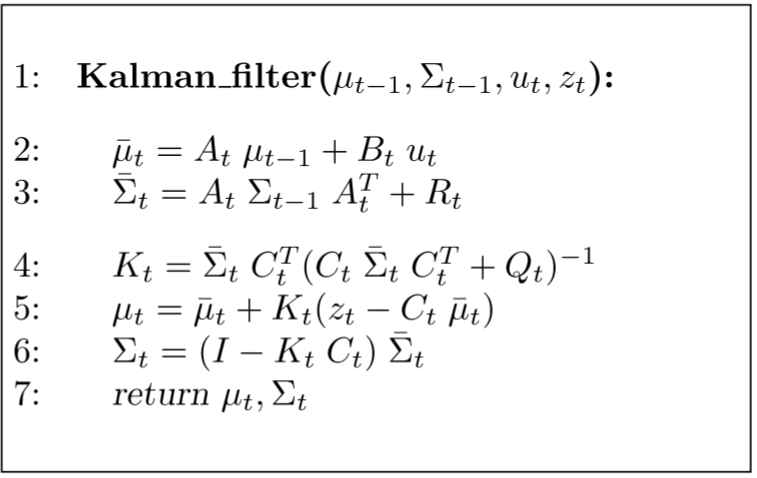
\includegraphics[width = 0.7\textwidth]{Kalman_Algoritme}
	\caption{Algoritme voor de Kalman filter \cite{Proballistic}}
	\label{kalman}
\end{figure}

\subsubsection{Extended Kalman filter}
De implementatie van de 'Extended Kalman filter' of EKF is een uitbreiding van de KF in de zin dat hierbij een niet-lineair model nu toch toegelaten is. Wanneer een niet lineair model toegepast wordt op de Bayes filter zou de kansverdeling voor de volgende toestand niet meer gaussisch zijn, ook al was de vorige dat wel. Dit komt omdat elke mogelijke positie binnen de verdeling anders verschaalt zou worden. Daarom moet het model gelineariseerd worden om toch nog de KF te kunnen gebruiken. Dit wordt uitgevoerd door rond de gemiddelde waarde te lineariseren. In een toestandsmodel betekent dit dus dat de Jacobiaan moet worden bepaald. \cite{controltheory}\\
Het algoritme voor de EKF ziet eruit zoals op figuur \ref{extkal}

\begin{figure}[h!]
	\centering
	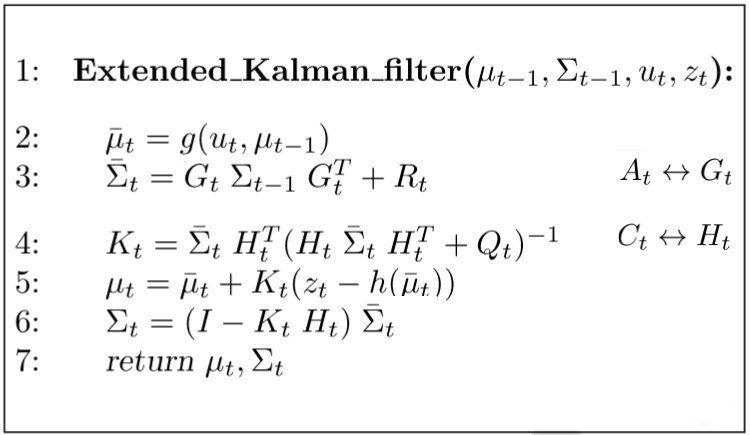
\includegraphics[width = 0.7\textwidth]{ExtendedKalman}
	\caption{Algoritme voor de Kalman filter \cite{Proballistic}}
	\label{extkal}
\end{figure}


\subsubsection{Unscented Kalman filter}
De 'Unscented Kalman filter' of UKF is op zijn beurt een uitbreiding van de EKF. Een niet-lineair model wordt opnieuw gelineariseerd maar nu niet meer rond het gemiddelde maar wel op basis van meerdere gewogen punten of sigma punten rond het gemiddelde. Op die manier kan een nauwkeurigere schatting gemaakt worden van de kansverdeling in de volgende toestand. Deze kansverdeling wordt wel nog steeds gaussisch beschouwd.\\
Een mogelijke strategie voor de keuze van deze sigma punten is om enerzijds het gemiddelde als punt te nemen en anderzijds voor elke dimensie van de gaussische verdeling twee extra punten, symmetrisch rond het gemiddelde. Voor de bepaling van de afstand waarop deze punten gekozen worden en het gewicht dat deze punten meekrijgen wordt verwezen naar het artikel \cite{unscented} uit de referenties. Het algoritme voor de UKF ziet er uit zoals op figuur \ref{unscented}



\begin{figure}[h!]
	\centering
	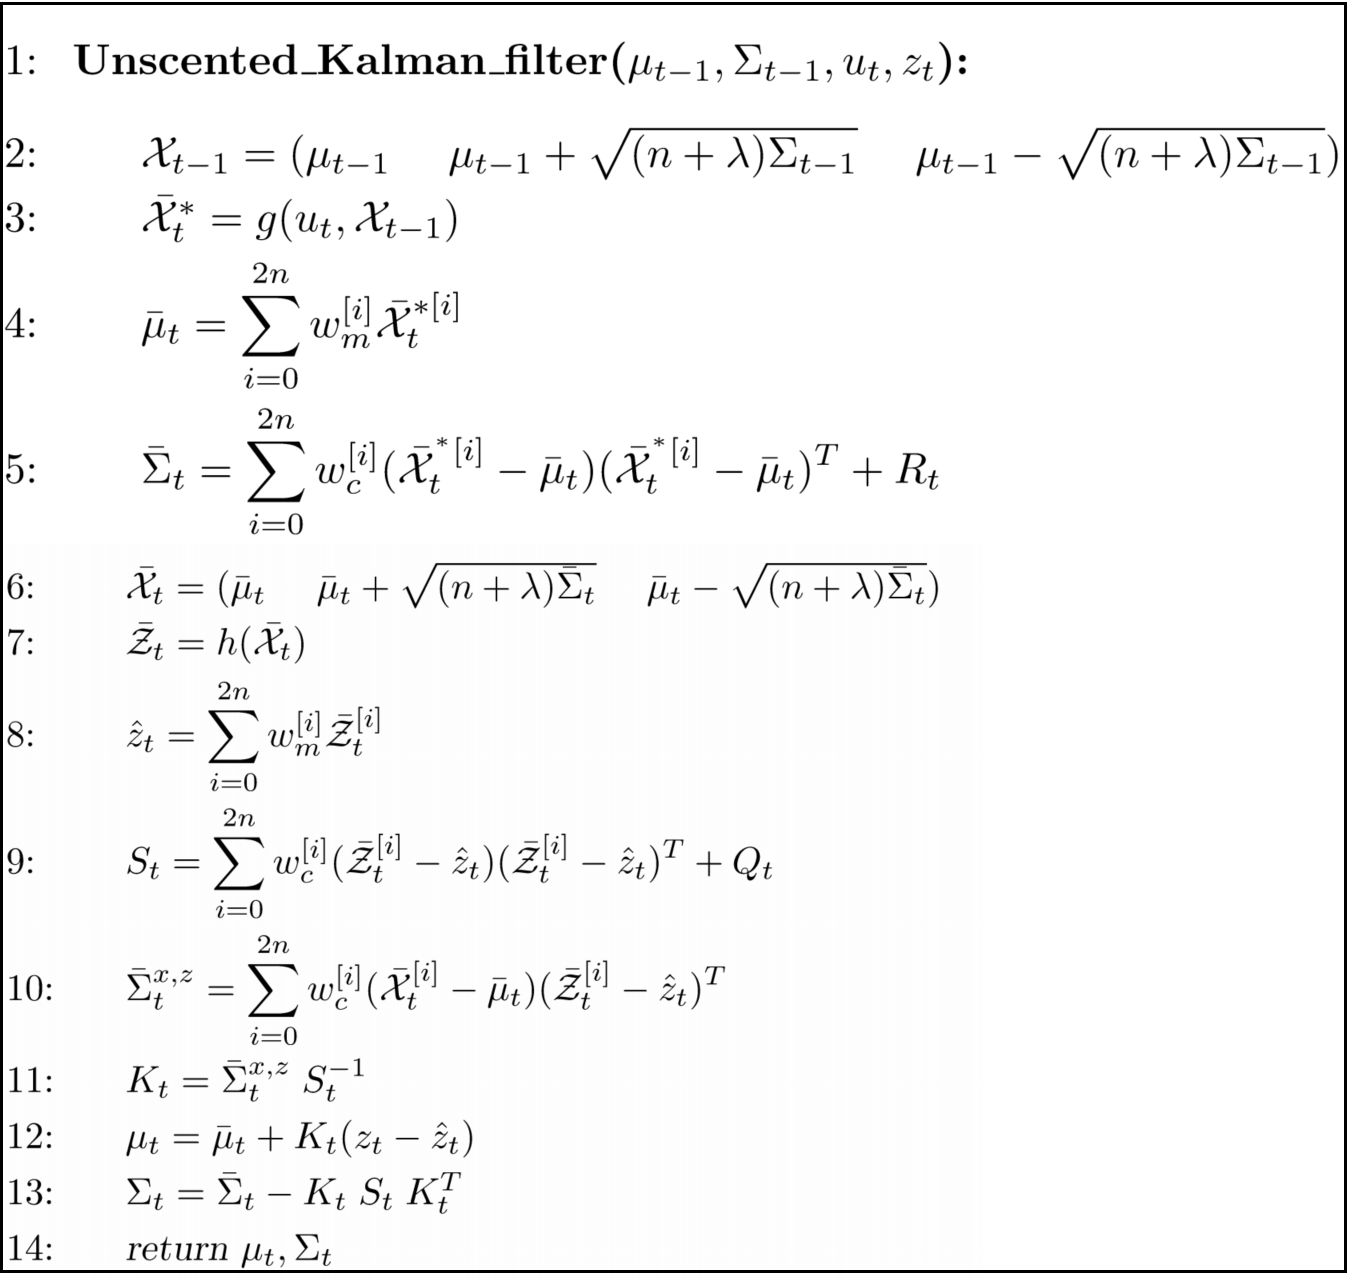
\includegraphics[width = 0.7\textwidth]{UnscentedKalman}
	\caption{Algoritme voor de UKF \cite{Course}}
	\label{unscented}
\end{figure}
Computationeel lijkt dit algoritme niet vereenvoudigd als men dit vergelijkt met de standaard KF aangezien nu wel in de correctiestap geen matrixinversie nodig is maar dan wel weer in de voorspellingsstap terwijl dit bij de KF omgekeerd is. 


\subsubsection{Extended information filter}
De 'information filter' of IF is opnieuw een implementatie van de KF met als grootste verschil dat er niet in het coördinatensysteem gewerkt wordt zoals beschreven in sectie \ref{beschrijving} maar dat deze vector getransformeerd wordt naar een ander coördinatensysteem. In deze implementatie wordt dan geen gebruik meer gemaakt van het gemiddelde $\mu$ en de covariantiematrix $\sum$ maar wel van de informatiematrix $\Omega$ en de informatievector $\xi$. Deze verhouden zich als:
\begin{equation}
\label{infor}
\begin{split}
\Omega = \Sigma^{-1} \\ \xi = \Sigma^{-1} \mu
\end{split}
\end{equation}
Wanneer dit ingevuld wordt in de implementatie van de KF zodat het gemiddelde en de covariantiematrix systematisch vervangen worden krijgt men :
\begin{figure}[h!]
	\centering
	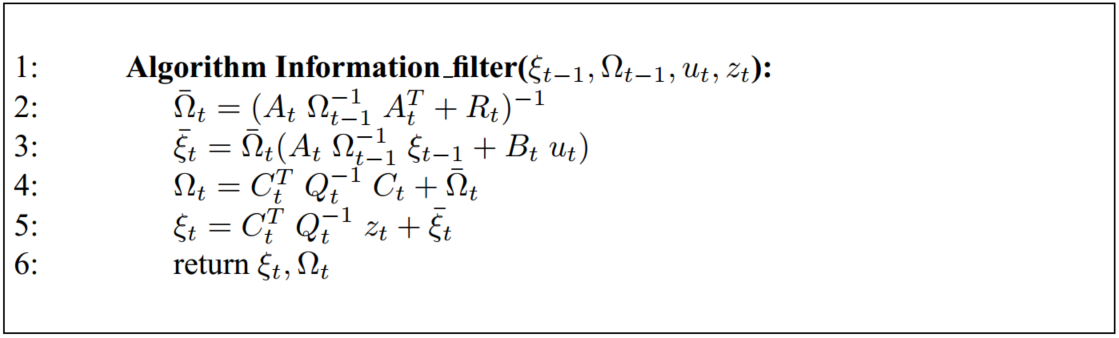
\includegraphics[width = \textwidth]{Information}
	\caption{Algoritme voor de IF \cite{Proballistic}}
	\label{information}
\end{figure}
Voor de afleiding hiervan wordt verwezen naar artikel \ref{Proballistic} van de referenties.\\
Voor niet-lineaire modellen bestaat ook voor deze implementatie de 'extendend information filter' of EIF. Gelijkaardig aan de EKF wordt voor deze implementatie ook een linearisatie gemaakt van het model. Het algoritme ziet er dan uit zoals in figuur \ref{extinf}

\begin{figure}[h!]
	\centering
	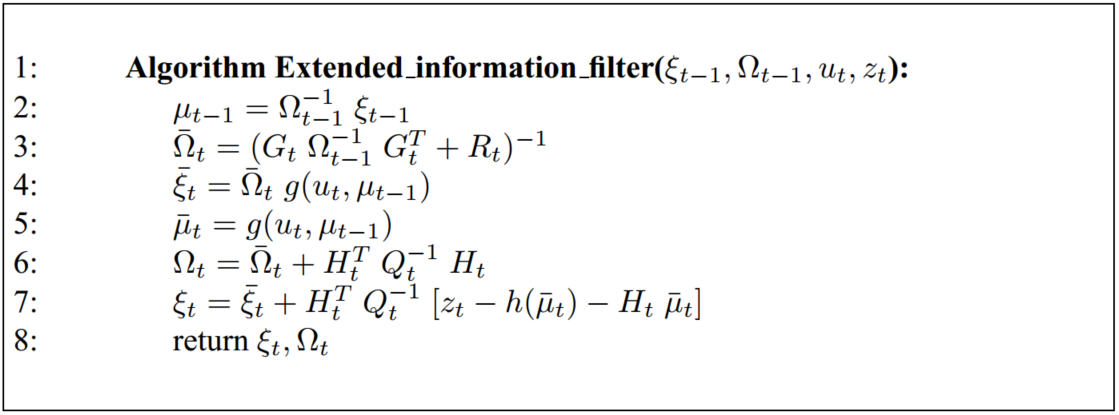
\includegraphics[width = \textwidth]{extinf}
	\caption{Algoritme voor de EIF \cite{Proballistic}}
	\label{extinf}
\end{figure}
Ook al lijkt de EIF computationeel niet efficiënter dan de EKF, aangezien er evenveel matrix-inversen nodig zijn, heeft deze toch een handige eigenschap. Als men de covariantiematrix vergelijkt met de genormaliseerde informatiematrix valt meteen op dat door de transformatie, de meeste elementen zich op de diagonaal bevinden. Dit wordt duidelijk op figuur \ref{sparse} waarop de donkerdere pixels grotere elementen voorstellen dan minder donkere. 

\begin{figure}[h!]
	\centering
	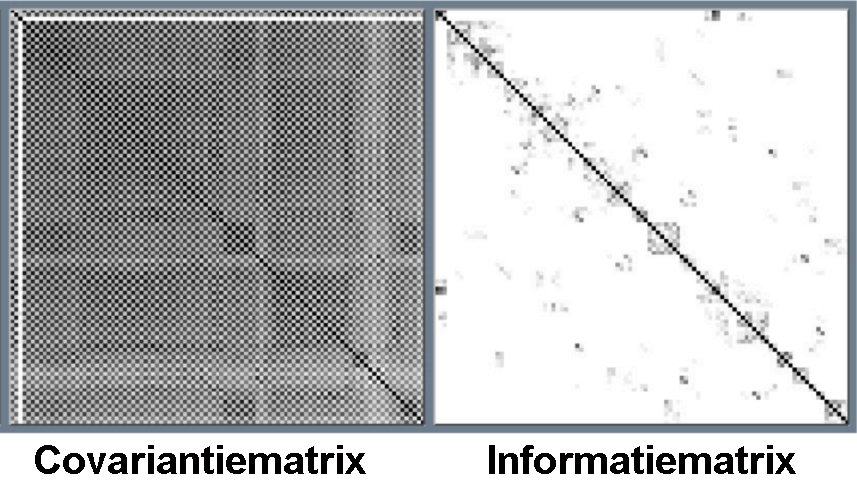
\includegraphics[width = 0.7\textwidth]{sparse}
	\caption{Het ijl karakter van de informatiematrix \cite{Course}}
	\label{sparse}
\end{figure}

Het ijl karakter van een matrix kan echter erg goed van pas komen wanneer deze geïnverteerd moet worden. Nu kunnen alle elementen van de informatiematrix buiten de diagonaal gelijk worden gesteld aan nul. Daardoor gaat wat informatie verloren, maar aangezien de meeste informatie geconcentreerd zit op de diagonaal wordt het verlies wel beperkt.\\
Voor hoge dimensies (veel objecten in de omgeving) kan het nu interessant zijn om gebruik te maken van de transformatie om de snelheid van het algoritme te verhogen.


\subsection{Particle filter}

De particle filter (PF) is een net als de KF een specifieke implementatie van de Bayes filter.
Het verschil tussen de KF en de PF is dat deze laatste de mogelijkheid heeft om met arbitraire kansverdelingen te werken. De KF was immers beperkt tot het gebruik van normaalverdelingen (gausscurve). Door een arbitraire kansverdeling $bel(x_{t})$ te bemonsteren ,wordt een groep monsters verkregen die deze kansverdeling benaderen. Dus in de plaats van de kansverdeling continu voor te stellen, stelt men hier de kansverdeling voor door een set monsters. Dit zorgt weliswaar voor een benadering, maar dit zorgt ervoor dat de verdeling die wordt verkregen niet-parametrisch is, en er dus veel meer verdelingen kunnen worden gebruikt.

Een monster $x_{t}^{[m]}$ ($1$ $\leqslant$ $m$ $\leqslant$ $M$), met $M$ het aantal monsters, is een bepaalde toestand waarin de robot zou kunnen verkeren op tijdstip $t$. Dit is dus een hypothese en niet de werkelijke toestand van de robot. Een toestand van de robot is bijvoorbeeld de positie waar de robot zich op dat moment bevindt.
Deze monsters kunnen gegroepeerd worden in een set 
\begin{equation}
\chi_{t} =x_{t}^{[1]}, x_{t}^{[2]},...,x_{t}^{[M]}
\end{equation}

Deze set $\chi_{t}$ wordt ook wel de particle set genoemd, waarbij een particle dus een ander benaming is voor een monster. In de tekst die volgt worden deze benamingen dan ook door elkaar gebruikt.

De kans dat een hypothese $x_{t}$ deel zal uitmaken van $\chi_{t}$ is gelinkt aan de bayes filter kansuitdrukking $bel(x_{t})$:
\begin{equation}
x_{t}^{[m]}  \sim p( x_{t} | z_{1:t}  ,  u_{1:t}) 
\end{equation}
Dit zorgt ervoor dat hoe meer particles min of meer dezelfde hypothetische toestand hebben, hoe groter de kans is dat de werkelijke toestand ongeveer die toestand zal zijn.

De particle set wordt opgebouwd op een recursieve manier, $\chi_{t}$ is gebaseerd op $\chi_{t-1}$. Het algoritme dat hiervoor instaat wordt weergegeven op figuur\ref{algoritmePF}. Dit algoritme is een speciale vorm van de PF, het is namelijk het algoritme met MCL aanpassing. Het verschil met het gewone algoritme wordt uitgelegd in sectie \ref{sampling}

\begin{figure}[H]
\centering
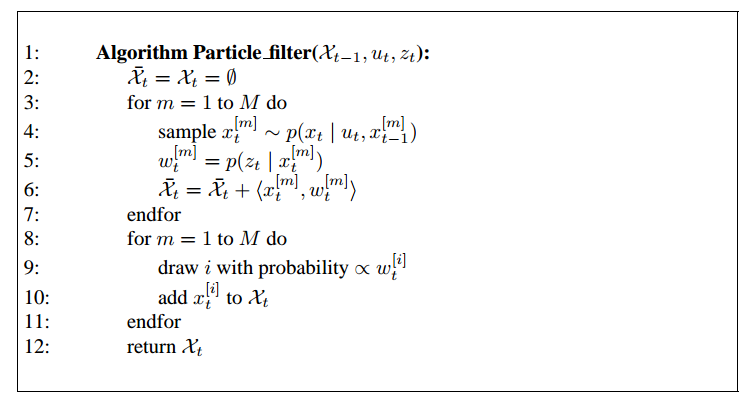
\includegraphics[width = 0.99\textwidth]{algoritmePF.png}
\caption{Algoritme voor opbouwen particle set}
\label{algoritmePF}
\end{figure}


Het algoritme genereert nieuwe mogelijke toestanden (dus nieuwe particles) voor één particle op basis van de controle signalen $u_{t}$ en de vorige hypothetische toestand van het particle (motion model). Anders gezegd neemt men de positie van het particle van de vorige tijdstap dan past men er de controlesignalen op toe en dan worden nieuwe samples gegenereerd rond deze nieuwe positie.
Daarna wordt bekeken of de nieuwe toestand overeenkomt met wat de robot observeert gegeven de robot zich zou bevinden in deze hypothetische toestand (observation model). Afhankelijk van hoe plausibel deze toestand is voor de werkelijkheid, wordt een gewicht $w_{t}^{[m]}$ gegeven aan het particle. Dit gewicht is een maat voor de belangrijkheid van het particle, als de toestand van het particle goed lijkt overeen te komen met de werkelijkheid krijgt het particle een hoog gewicht.
De particles, samen met hun gewicht, worden voorlopig opgeslaan in $\overline{\chi_{t}}$. Deze set monsters geeft eigenlijk $\overline{bel}(x_t)$ weer (prediction step).Daarna worden particles getrokken uit  $\overline{\chi_{t}}$, deze actie wordt herbemonsteren genoemd. Hoe groter het gewicht van de particles, hoe groter de kans dat de particles getrokken worden. De getrokken particles worden daarna in de definitieve particle set $\chi_{t}$ gezet. Deze particle set geeft na het herbemonsteren $bel(x_{t})$ weer (correction step), aangezien hier de observaties (gerelateerd met gewicht) worden meegenomen in de keuze van de samples.

\subsubsection{Sampling}
\label{sampling}
Aangezien de kern van de PF nu net gaat over monsters van een kansverdeling, moeten er dus bemonsterd worden om een set monsters te bekomen. Samplen van een arbitraire distributie, target distribution $f$ genoemd, is echter niet altijd mogelijk. Als oplossing wordt een andere kansverdeling bemonsterd die bemonsterbaar is, de proposal distribution $g$ genoemd. Voor deze verdeling wordt veelal de gausscurve gebruikt. Waarbij $f$ overeenkomt met $bel(x_{t})$ en $g$ overeenkomt met $\overline{bel}(x_{t})$. Door voor elk monster de kans van de target distribution te delen door de kans van de proposal distribution wordt een gewicht bekomen:

\begin{equation}
w^{[m]}=\dfrac{f(x_{[m]})}{g(x^{[m]})}
\label{gewicht}
\end{equation}

Op deze manier kan er dus worden gesampled en tegelijk een gewicht meegegeven worden aan de samples \ref{samples1} en \ref{samples2}.
Bij MCL, een speciale vorm van de PF, wordt voor de proposal distribution het motion model gekozen. Dit is te zien op lijn vier van het algoritme op figuur\ref{algoritmePF}. Op lijn vijf neemt men het gewicht gelijk aan het observation model, indien de proposal het motion model is. Dit laatste wordt aangetoond in sectie SECTIE REFEREREN GVD!!!!!!!!!!!




\begin{multicols}{2}
	\begin{figure}[H]
	\centering
	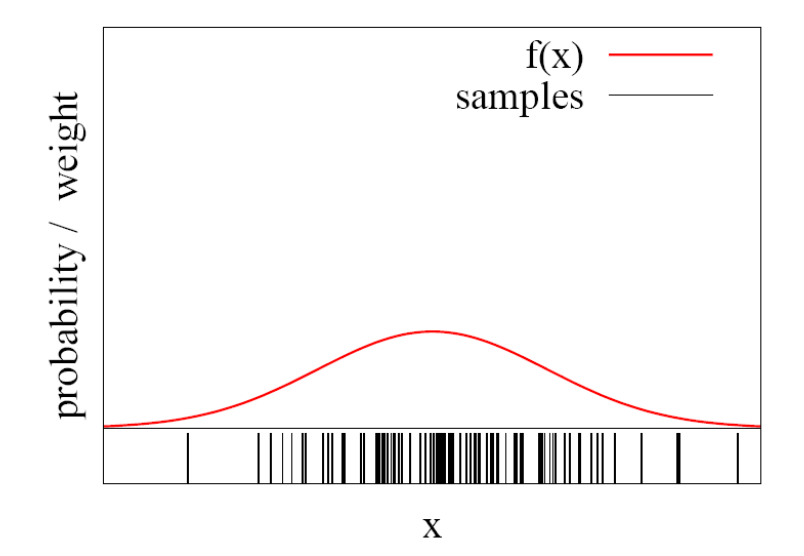
\includegraphics[width = 0.45\textwidth]{samples.png}
	\caption{Bemonstering van proposal distribution}
	\label{samples1}
	\end{figure}
	
	\begin{figure}[H]
	\centering
	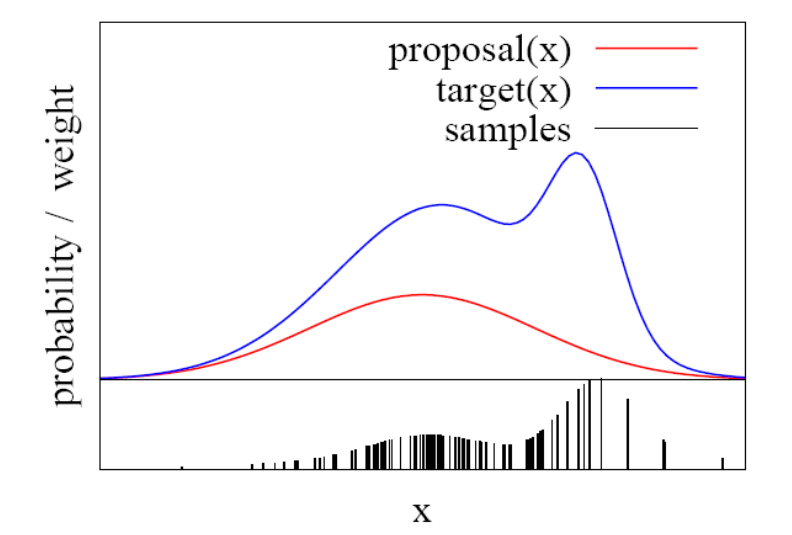
\includegraphics[width = 0.45\textwidth]{samples2.png}
	\caption{Bemonstering van target distribution}
	\label{samples2}
	\end{figure}
\end{multicols}


\subsubsection{Gewichten voor Monte Carlo Localization}
In deze sectie bewijzen we de bewering gemaakt in sectie\ref{sampling} dat indien de proposal distribution gelijk wordt genomen aan het motion model, dan de gewichten evenredig zijn met het observation model.


Ieder particle is een geschiedenis van hypothetische toestanden waarin de robot zou zijn geweest. Deze toestanden zijn, zoals bovenvermeld, in MCL de posities van de robot. Een particle bevat dus eigenlijk een hypothese van het traject dat de robot heeft doorlopen. De PF berekent dus eigenlijk $p(x_t|z_{1:t},u_{1:t})$ maar dan over alle toestanden van de robot:

\begin{equation}
bel(x_{0:t})= p(x_{0:t}| u_{1:t},z_{1:t})
\end{equation}

Analoge afleiding van sectie (DEJENSN ZIJN AFLEIDINGE) toegepast op $bel(x_{0:t})$ levert volgende uitdrukking op (met assumptie van oneindig veel particles):
\begin{equation}
bel(x_{0:t})= p(x_{0:t}| u_{1:t},z_{1:t}) = \eta p(z_{t}|x_{t}) p(x_{t}|x_{t-1},u_{t}) p(x_{0:t-1}|z_{1:t-1},u_{1:t-1})
\label{target}
\end{equation}

Zoals bovenvermeld komt de proposal overeen met $\overline{bel}(x_{t})$, namelijk het motion model samen met een recurieve term:
\begin{equation}
\overline{bel}(x_{t})=p(x_{t}|x_{t-1},u_{t})bel(x_{0:t-1})=p(x_{t}|x_{t-1},u_{t})p(x_{0:t-1}|z_{1:t-1},u_{1:t-1})
\label{prop}
\end{equation}

vergelijkingen \ref{target} en \ref{prop} invullen in vergelijking\ref{gewicht} geeft

\begin{equation}
w_{t}^{[m]}= \dfrac{\eta p(z_{t}|x_{t}) p(x_{t}|x_{t-1},u_{t}) p(x_{0:t-1}|z_{1:t-1},u_{1:t-1})}{p(x_{t}|x_{t-1},u_{t})p(x_{0:t-1}|z_{1:t-1},u_{1:t-1})}
\end{equation}
 
met als resultaat:
\begin{equation}
w_{t}^{[m]}= \eta p(z_{t}|x_{t})
\label{gewichten}
\end{equation}

In vergelijking\ref{gewichten} zien we dat de gewichten gelijk zijn aan het observation model.
Merk op dat door te herbemonsteren met gewichten $w_{t}^{[m]}$, de overblijvende monsters in $/chi_{t}$ verdeeld zijn volgens het product van de proposal en de gewichten:
\begin{equation}
bel(x_{0:t})= \eta w_{t}^{[m]} p(x_{t}|x_{t-1},u_{t}) p(x_{0:t-1}|z_{1:t-1},u_{1:t-1})
\end{equation}


\subsubsection{Voor-en nadelen van de implementatie}
\paragraph{Voordelen}
\begin{itemize}
\item Er kunnen niet-parametrische target distributions worden gebruikt.
\item Er kan geen foute data-associatie gebeuren, wat bij de KF wel kan. De reden hiervoor is dat indien de robot bijvoorbeeld 2 of meer plausibele toestanden van de werkelijkheid heeft, er tussen deze toestanden niet wordt gekozen. Ze worden immers allebei gekozen, door beide toestanden te bemonsteren. Wanneer men verdergaat in de tijd en de robot dus heeft bewogen, zullen er bepaalde toestanden minder waarschijnlijk worden en zullen deze verdwijnen. Vergelijk het met dat er op de wereld 2 exact dezelfde straten zouden zijn in een verschillende stad , dan worden deze 2 straten bemonsterd. Wanneer de robot beweegt doorheen de straat en uiteindelijk in een andere straat terechtkomt, zal in 1 van de twee straten de observatie niet overeenkomen met de map die reeds werd gemaakt, dan weet men dat men zich in de andere straat bevindt.  
\end{itemize}

\paragraph{Nadelen}
\begin{itemize}
\item Er zijn veel particles nodig zodat deze monsters de gewenste target distribution goed weergeven.
\item Wanneer men bij MCL met sensoren werkt die zeer accuraat zijn ($p(z|x)$ is bijna een dirac-distributie), dan kan het zijn dat het motion model (de proposal) geen samples genereert op de plaatsen in het gebied waar p(z|x) >0. Dit zorgt ervoor dat alle gewichten nul zijn, en geeft dus problemen wanneer er moet herbemonsterd worden.
\item Werkt het best als de toestandsvector laag-dimensioneel is. Aangezien een particle een hypothese is voor een toestand, zijn er minder particles nodig voor een toestand te beschrijven met een weinig aantal dimensies dan een toestand met veel dimensies. 
\label{nadelen}
\end{itemize}

\subsubsection{Mapping}
Indien er naast de positie van de robot ook de posities van de landmarks zouden worden meegenomen in de toestandsvector, dan zou de toestandsvector hoog-dimensioneel worden. Dit is zoals gezegd in sectie \ref{nadelen} niet gewenst.
De oplossing hiervoor is om een verband te zien tussen de positie van de robot en de landmarks, namelijk eens je de positie van de robot weet, is het makkelijk om de omgeving in kaart te brengen. Want eenmaal je het traject van de robot weet, kan je de positie van de landmarks updaten met de verkregen observaties van de sensoren.
De idee is dus om met de PF de poses van de robot te bepalen. Elk sample heeft een eigen traject, en dus een eigen map die verschillend is van de andere particles. Aan ieder traject hangt dus een bepaalde map en die map is het resultaat van het traject die werd afgelegd.

Het principe van Rao-Blackwellization kan men als volgt samenvatten in formules:
\begin{equation}
p(a,b) = p(b|a) p(a)
\label{rao}
\end{equation}
Waarbij $a$ het traject van het particle voorstelt en $b$ de map voorstelt. De eerste factor p(b|a) kan efficiënt berekent worden voor elk sample en p(a) stelt de samples voor, namelijk $bel(x_{0:t})$. Anders gezegd kunnen we vergelijking \ref{rao} ook voorstellen als:
\begin{equation}
p(x_{0:t},m_{1:M}|z_{1:t},u_{1:t})= p(m_{1:M}|x_{0:t},z_{1:t})p(x_{0:t}|z_{1:t},u_{1:t}) 
\end{equation}
Waarbij dus de eerste factor $p(m_{1:M}|x_{0:t},z_{1:t})$ de map opbouwd op basis van het traject en de observaties en de tweede factor $p(x_{0:t}|z_{1:t},u_{1:t})$ het traject voorstelt, merk op dat $m{1:M}$ hier de map voorstelt op basis van landmarks, met $M$ het aantal landmarks.
Om de PF computationeel mogelijk te maken is het de bedoeling dat wanneer er een traject van het particle dus voorhanden is er efficiënt een map van dat particle kan worden opgebouwd. Alle landmarks zijn onafhankelijk van elkaar als je het traject van de robot kent (CYRILL STACHNISS ZEGT DA, LECTURE 12 minuut 20:08). Dit zorgt ervoor dat je de factor die de map met landmarks berekent kunt opsplitsen in een product dat één enkel landmark berekent. Hierbij stellen de factoren $p(m_{i}|x_{0:t},z_{1:t})$ onafhankelijke gaussische distributies voor, dit geeft:
\begin{equation}
p(x_{0:t},m_{1:M}|z_{1:t},u_{1:t})= \prod_{i=1}^Mp(m_{i}|x_{0:t},z_{1:t})p(x_{0:t}|z_{1:t},u_{1:t}) 
\end{equation}
De map wordt nog steeds gemaakt zoals in de methode van de EKF, dit komt erop neer dat er in de plaats van een hoog dimensionele EKF, moet er een kleine 2x2 EKF worden opgelost voor elk landmark. Elk particle heeft dus een 2x2 EKF dat het moet oplossen voor de bepaling van ieder landmark, wat zeer efficiënt is. De keerzijde is dat dit wel voor ieder particle moet gebeuren, maar toch is dit nog efficiënter dan indien er een hoog dimensionele EKF zou moeten worden opgelost. (DA BENK IER NIE GJIL ZEKER, zie cyrill 22:24 les 12) 

\subsection{FastSLAM}
\subsubsection{FastSLAM 1.0}
Fastslam is de implementatie van de PF in combinatie met de mapping adh van Rao-Blackwellization. Hier wordt wel niet het volledige traject meegenomen maar enkel de huidige positie. Dit komt omdat wanneer de robot verder beweegt in de tijd we nooit terugkeren naar een bepaalde toestand vroeger om bijvoorbeeld de positie ervan te corrigeren. De PF kijkt altijd in de toekomst om de positie in de volgende tijdstap te berekenen. Het is de bedoeling dat er wel online, dus voor iedere tijdstap een huidige map wordt gemaakt die ergens wordt weggeschreven. Een particle houdt dus de positie bij waarop het zich op dat moment bevindt en ieder landmark wordt voorgesteld door een 2x2 EKF, zie figuur\ref{algoritmePF}.

\begin{figure}[H]
\centering
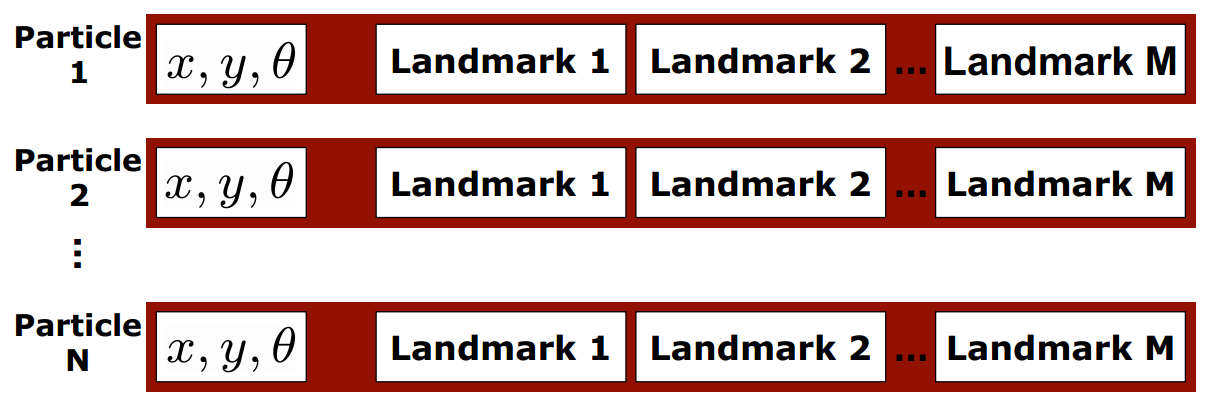
\includegraphics[width = 0.99\textwidth]{fastslam.png}
\caption{Particles bevatten hun positie en 2x2 EKF voor de voorstelling van ieder landmark}
\label{fastslam}
\end{figure}
%%FIGUUR :http://ais.informatik.uni-freiburg.de/teaching/ws13/mapping/pdf/slam12-fastslam.pdf

\subsubsection{FastSLAM 2.0}
Het verschil met Fastslam 1.0 is om naast enkel de odometry te gebruiken voor het bepalen van de volgende toestand er nu ook rekening wordt gehouden met sensor informatie in de proposal distribution. Dit zorgt ervoor dat meer samples beter zullen aansluiten bij de target distribution. Dit zorgt er voor dat er minder particles nodig zijn en dat de map nauwkeuriger zal zijn.



\subsubsection{Grid-Based FastSLAM}
Dit is een particle gebaseerd SLAM algoritme voor het maken van grid-maps. Het voordeel is dat er geen feature moet worden ingebouwd om data-associatie te verwezenlijken tussen de landmarks en er dus geen foute data-associatie kan gebeuren. 
Grid-Based SLAM maakt gebruikt van het principe van FastSLAM 2.0 omdat er hier landmarks zijn waarbij de robot deze bij de measurement update kan corrigeren. Een grid map waarbij het traject niet heel correct is, is minder goed dan een landmark gebaseerde map voor navigatie.
De observatie die wordt meegenomen in de proposal distribution is een zogenaamde scan-matcher. Hierbij wordt de kans gemaximaliseerd dat deze huidige map en positie relatief overeenkomt met de vorige map en positie. Anders gezegd neemt men de map van de vorige positie en de observatie van de huidige positie en verschuift men (roteren,transleren) de map zodat de huidige map het best overlapt met de vorige map. In formule wordt dit als volgt weergegeven:

\begin{equation}
x_{t}^{*}=\underset{x_{t}}{argmax}\{p(z_{t}|x_{t},m_{t-1})p(x_{t}|u_{t-1},x_{t-1}^{*}) \}
\end{equation}

Mathematisch gezien is dit niet volledig correct, aangezien de observatie al reeds wordt gebruikt in de proposal distribution. Dit zorgt ervoor dat de berekening voor de gewichten zou moeten worden aangepast.
Als oplossing hiervoor wordt niet alles gescanmatched, maar enkel bepaalde blokken van bijvoorbeeld 100 posities. Als resultaat krijg je voor die 100 posities een locale map die nauwkeurig is, en dan gebruik je de scanmatcher om deze lokale mappen te laten overlappen.






\subsection{Graph-Based SLAM}
Graph-Based SLAM is een methode die niet gebaseerd is op de recursieve Bayes filter maar eerder op een graaf-voorstelling van het probleem. Elke knoop stelt een positie voor terwijl de verbindingen tussen de knopen staan voor randvoorwaarden tussen de twee knopen. Deze kunnen enerzijds afkomstig zijn van het bewegingsmodel waarin de voorspelling gemaakt wordt op basis van de besturingscommando's (e: odometry). Anderzijds kunnen ook randvoorwaarden opgelegd worden op basis van de observaties. Hiervoor worden observaties van de ene toestand vergeleken met die van de volgende toestand en wordt gezocht naar maximaal overlap. Op basis daarvan kan dan een andere voorspelling gemaakt worden van de volgende toestand, en meteen ook de relatieve relatie volgens de observaties tussen deze twee toestanden gedefinieerd worden.\\
Zo'n verbinding stelt dus eigenlijk een kansverdeling van de relatieve positie tussen de twee knopen voor aangezien in beide modellen ook de variantie opgenomen is. In een ééndimensionale omgeving zou dit dus de waarschijnlijkheid voor de afstand tussen de twee knopen volgens de hoofdas zijn. 
%Omdat vanuit een knoop in het algemene geval meerdere knopen waargenomen kunnen worden is de verdeling van het observatiemodel niet gaussisch maar wel multimodaal. Om toch de complexiteit in de hand te houden wordt in praktische implementaties de meest waarschijnlijke topologie bepaald en de verdeling beperkt zodat deze gaussich kan worden beschouwd. 
Door nu voor elke knoop de voorspelling op basis van het bewegingsmodel $\hat{z}_{ij}$ te vergelijken met de voorspelling op basis van het observatiemodel $z_{ij}$ kan een foutenfunctie bepaalt worden voor elke knoop als volgt:
\begin{equation}
e_{ij}(x_i,x_j) = z_{ij} - \hat{z}_{ij}(x_i,x_j)
\end{equation}
Door dit voor elke observatie te doen kan vervolgens een foutenfunctie opgesteld worden:
\begin{equation}
F(x) = \sum\limits_{(i,j)} e_{ij}^T \Omega_{ij} e_{ij}
\end{equation}
waarbij $\Omega_{ij}$ als gedefinieerd in (\ref{infor}). Hiervoor wordt verondersteld dat alle observaties onafhankelijk zijn van elkaar. Hiermee moet dan ook rekening gehouden worden bij het implementeren van de manier van observeren. Zodat niet twee keer na elkaar dezelfde observatie wordt gedaan als de robot niet beweegt bijvoorbeeld. Door deze foutenfunctie te minimaliseren wordt de kans gemaximaliseerd of vindt men dus het gemiddelde. Een manier om dat te doen wordt aangereikt in sectie IV. A in \cite{graph} van de referenties.\\
Als een toestand bepaalt wordt is dat altijd gerefereerd naar de vorige positie. Dit betekent dat hier geen globaal assenstelsel gedefinieerd is aangezien het telkens om de relatieve positie tussen de twee toestanden gaat. \\
\subsubsection{Het algoritme}\cite{graph}
Telkens wanneer de robot begint te bewegen en een bepaalde ondergrens van beweging overschrijdt (bijvoorbeeld 0.5 meter vooruit), wordt een nieuwe toestand gegenereerd in de graaf. M.b.v. de informatie uit de beweginscommando's kan onmiddellijk ook schatting gemaakt worden van de volgende toestand. Dit betekent dat er een extra randvoorwaarde, of dus een verbinding met de vorige toestand, gemaakt wordt in de graaf. Als de robot later in een gebied terugkeert waar hij reeds geweest is zoekt deze naar gelijkenissen tussen de huidige observaties en vorige observaties die in aanmerking komen (door bijvoorbeeld terugrekenen van het bewegingsmodel). De beste gelijkenis wordt dan zo goed mogelijk gepast op de huidige waardoor weer een nieuwe randvoorwaarde toegevoegd wordt. Deze randvoorwaarde komt neer op een verbinding in de graaf tussen de huidige toestand en één van de vorige toestanden. De toevoeging van deze randvoorwaarde beïnvloed ook alle vorige toestanden en bouwt extra zekerheid in de map en over de vorige toestanden. Dit wordt het sluiten van een lus genoemd en is essentieel in deze implementatie. Hoe vaker een lus gesloten kan worden, hoe meer zekerheid ingebouwd kan worden.  
\subsubsection{Hierarchical Pose-Graph} 
Een belangrijke opmerking bij deze methode is dat het stelsel dat opgelost moet worden groeit voor elke randvoorwaarde die er bij komt. Dit betekent dat er een punt komt waarop het stelsel niet meer opgelost kan worden binnen de tijd tussen twee toestanden. % ksnap et nog niet dus lat u gerust gaan











\end{document}
